\documentclass[tikz, border=10pt]{standalone}
\usepackage{tikz}
\usepackage{amsmath}
\usetikzlibrary{arrows.meta, shapes.geometric, positioning, fit, backgrounds}

\begin{document}
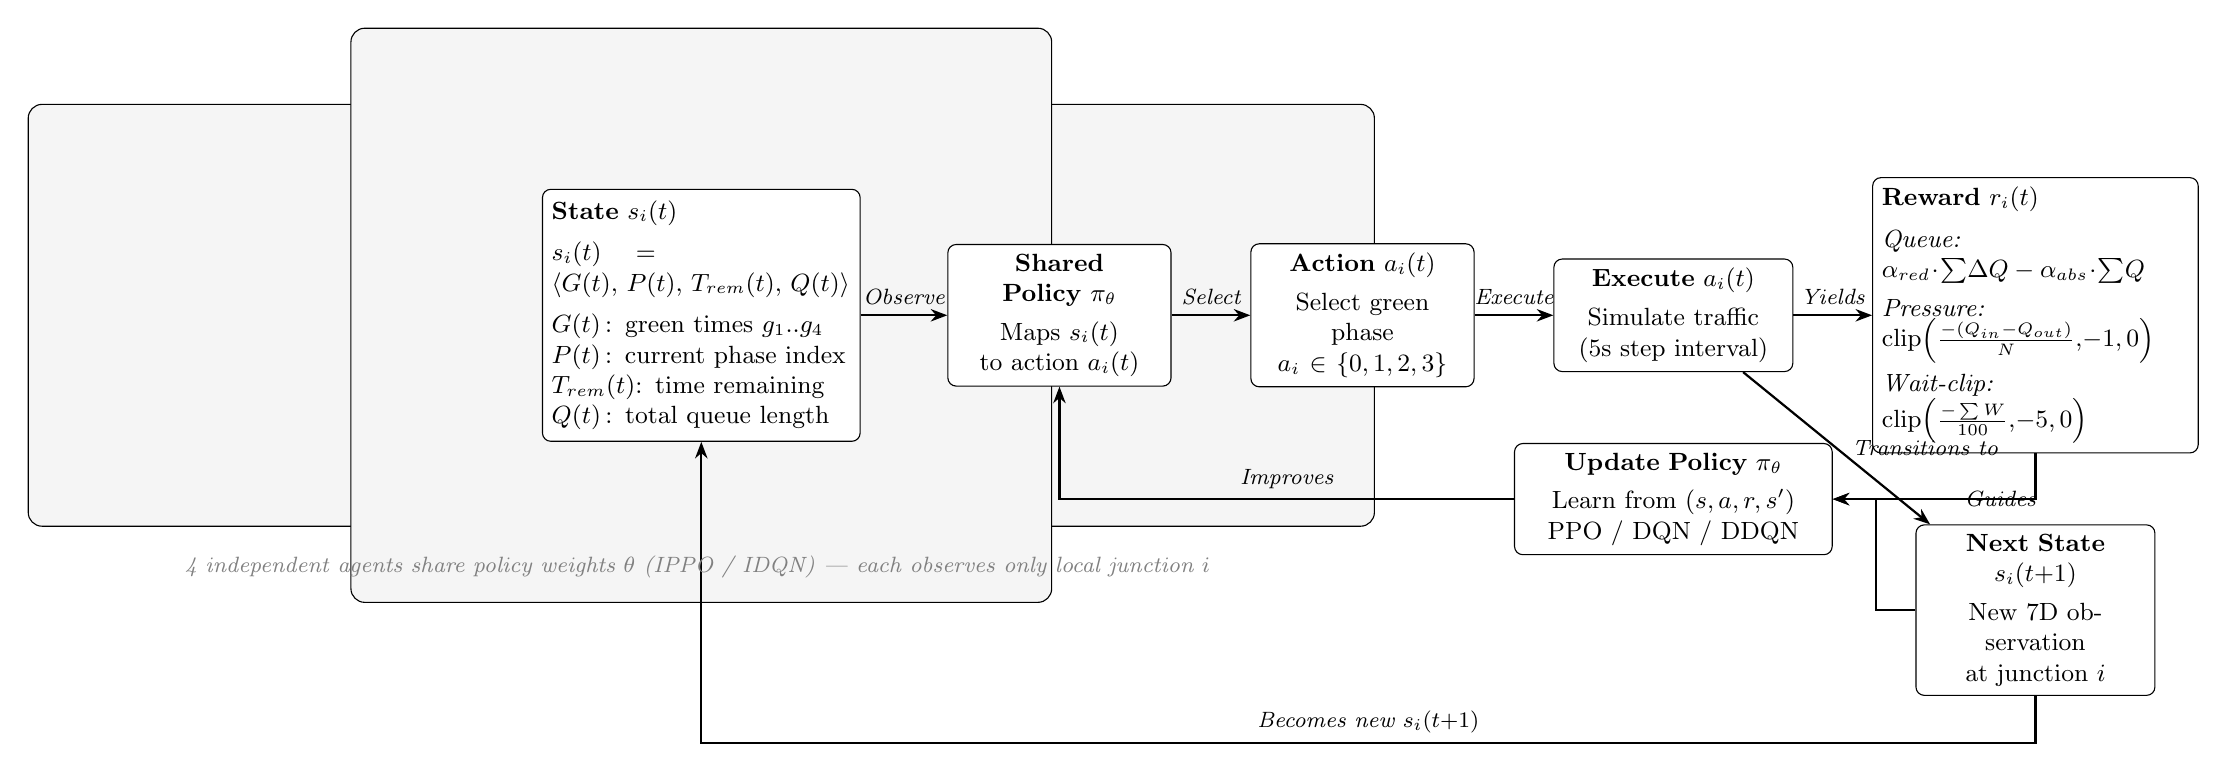
\begin{tikzpicture}[
    box/.style={
        rectangle, draw, rounded corners=3pt,
        text centered, minimum height=1.0cm,
        font=\small, fill=white
    },
    bigbox/.style={
        rectangle, draw, rounded corners=5pt,
        font=\small\bfseries, fill=gray!8,
        inner sep=10pt
    },
    arrow/.style={-{Stealth[length=6pt]}, thick},
    dasharrow/.style={-{Stealth[length=6pt]}, thick, dashed},
    label/.style={font=\footnotesize\itshape, midway}
]

%% ─── LEFT BLOCK: Traffic Controller ──────────────────────────
\node[box, text width=3.8cm, align=left, minimum height=3.2cm] (state) at (0,0) {
    \textbf{State $s_i(t)$} \\[4pt]
    $s_i(t) = \langle G(t),\, P(t),\, T_{rem}(t),\, Q(t) \rangle$ \\[4pt]
    $G(t)$\,: green times $g_1..g_4$ \\
    $P(t)$\,: current phase index \\
    $T_{rem}(t)$: time remaining \\
    $Q(t)$\,: total queue length
};

\node[box, text width=2.6cm, align=center, minimum height=1.4cm,
      right=1.1cm of state] (policy) {
    \textbf{Shared Policy} $\pi_\theta$ \\[3pt]
    Maps $s_i(t)$ \\
    to action $a_i(t)$
};

\node[box, text width=2.6cm, align=center, minimum height=1.4cm,
      right=1.0cm of policy] (action) {
    \textbf{Action $a_i(t)$} \\[3pt]
    Select green phase \\
    $a_i \in \{0, 1, 2, 3\}$
};

%% ─── RIGHT BLOCK: SUMO Environment ───────────────────────────
\node[box, text width=2.8cm, align=center, minimum height=1.4cm,
      right=1.0cm of action] (execute) {
    \textbf{Execute $a_i(t)$} \\[3pt]
    Simulate traffic \\
    (5s step interval)
};

\node[box, text width=3.9cm, align=left, minimum height=3.4cm,
      right=1.0cm of execute] (reward) {
    \textbf{Reward $r_i(t)$} \\[4pt]
    \textit{Queue:} \\
    $\alpha_{red}\!\cdot\!\sum\!\Delta Q - \alpha_{abs}\!\cdot\!\sum\!Q$ \\[3pt]
    \textit{Pressure:} \\
    $\text{clip}\!\left(\frac{-(Q_{in}-Q_{out})}{N},\!-1,0\right)$ \\[3pt]
    \textit{Wait-clip:} \\
    $\text{clip}\!\left(\frac{-\sum W}{100},\!-5,0\right)$
};

\node[box, text width=2.8cm, align=center, minimum height=1.2cm,
      below=0.9cm of reward] (nextstate) {
    \textbf{Next State $s_i(t{+}1)$} \\[3pt]
    New 7D observation \\
    at junction $i$
};

%% ─── BOTTOM: Update ──────────────────────────────────────────
\node[box, text width=3.8cm, align=center, minimum height=1.2cm,
      below=0.9cm of execute] (update) {
    \textbf{Update Policy $\pi_\theta$} \\[3pt]
    Learn from $(s,a,r,s')$ \\
    \small PPO / DQN / DDQN
};

%% ─── OUTER FRAMES ─────────────────────────────────────────────
\begin{scope}[on background layer]
  % Left frame — Traffic Controller
  \node[bigbox, fit=(state)(policy)(action)(update),
        label={[anchor=north west]north west:\textbf{Traffic Controller (Agent $i$)}}
       ] (leftframe) {};

  % Right frame — SUMO
  \node[bigbox, fit=(execute)(reward)(nextstate),
        label={[anchor=north west]north west:\textbf{SUMO Environment}}
       ] (rightframe) {};
\end{scope}

%% ─── ARROWS ──────────────────────────────────────────────────
\draw[arrow] (state)     -- node[above, font=\footnotesize\it]{Observe} (policy);
\draw[arrow] (policy)    -- node[above, font=\footnotesize\it]{Select}  (action);
\draw[arrow] (action)    -- node[above, font=\footnotesize\it]{Execute} (execute);

% Execute → Reward (yields)
\draw[arrow] (execute)   -- node[above, font=\footnotesize\it]{Yields}  (reward);

% Execute → NextState (transitions)
\draw[arrow] (execute)   -- node[right, font=\footnotesize\it, xshift=2pt]{Transitions to} (nextstate);

% NextState → state (becomes new, bottom loop)
\draw[arrow] (nextstate.south) -- ++(0,-0.6)
    -| node[above, font=\footnotesize\it, pos=0.25]{Becomes new $s_i(t{+}1)$}
    (state.south);

% Reward + NextState → update
\draw[arrow] (reward.south)    |- node[right, font=\footnotesize\it, pos=0.7]{Guides} (update.east);
\draw[arrow] (nextstate.west)  -- ++(-0.5,0) |- (update.east);

% Update → Policy (improves)
\draw[arrow] (update.west) -- node[above, font=\footnotesize\it]{Improves} (policy.south |- update.west)
    -- (policy.south);

%% ─── Multi-agent note ────────────────────────────────────────
\node[font=\footnotesize, align=center, text=gray,
      below=0.25cm of leftframe.south] {
    \textit{4 independent agents share policy weights $\theta$ (IPPO / IDQN) — each observes only local junction $i$}
};

\end{tikzpicture}
\end{document}
